\documentclass[12pt,a4paper]{article}
\usepackage{t1enc}
\usepackage{amsmath}
\usepackage[european]{circuitikz}
\usepackage{listings}
\usepackage{color}
\usepackage{graphicx}
\usepackage{float}
\usepackage{hyperref}
\usepackage{geometry}
\usepackage[hungarian]{babel}
\definecolor{mygreen}{rgb}{0,0.6,0}
\definecolor{mygray}{rgb}{0.5,0.5,0.5}
\definecolor{mymauve}{rgb}{0.58,0,0.82}
\setcounter{secnumdepth}{2}

% Geometry settings
\geometry{
    a4paper,
    left=25mm,
    right=25mm,
    top=25mm,
    bottom=25mm
}

\ctikzset{inductor = american}

\lstset{
    backgroundcolor=\color{white},
    basicstyle=\footnotesize,
    breakatwhitespace=false,
    breaklines=true,
    captionpos=b,
    commentstyle=\color{mygreen},
    escapeinside={\%*}{*)},
    extendedchars=true,
    frame=single,
    keepspaces=true,
    keywordstyle=\color{blue},
    language=Matlab,
    numbers=left,
    numbersep=5pt,
    numberstyle=\tiny\color{mygray},
    rulecolor=\color{black},
    showspaces=false,
    showstringspaces=false,
    showtabs=false,
    stepnumber=1,
    stringstyle=\color{mymauve},
    tabsize=2,
    title=\lstname
}

\hypersetup{
    colorlinks=true,
    linkcolor=black,
    citecolor=black,
    filecolor=black,
    urlcolor=black,
    pdfborder={0 0 0}
}

\begin{document}

% Cover Page
\begin{titlepage}
    \centering
    \vspace*{\fill}
    \textbf{\Huge Parametrikus oszcillátor szimulációja}\\[2cm]
    \includegraphics[width=0.65\textwidth]{figures/bme_logo_nagy_bordo.jpg}\\[1cm]
    \textbf{\Large Budapest Műszaki és Gazdaságtudományi Egyetem}\\[0.25cm]
    \Large Villamosmérnöki és Informatikai Kar\\[1cm]
    \includegraphics[width=0.2\textwidth]{figures/hvt-logo.png}\\[0.25cm]
    \Large Szélessávú Hírközlés és Villamosságtan Tanszék\\[2cm]
    \Large IMSC Házi feladat\\[0.25cm]
    \Large Jelek és rendszerek 2 (BMEVIHVAB02 2024/25/1)\\[1.5cm]
    \Large \textbf{\textit{Szerző:}}\\[0.25cm]
    \Large Kovács Levente (F5UHYT)\\[1cm]
    \small \textit{Konzulens:}\\[0.25cm]
    \small Dr. Gyimóthy Szabolcs\\[2cm]
    \Large \today
    \vspace*{\fill}
\end{titlepage}
\newpage

% Page numbering
\pagenumbering{arabic}
% Table of Contents
\tableofcontents
\newpage

\begin{abstract}
    A parametrikus oszcillátorok olyan rendszerek, amelyekben az egyik vagy több paraméter időben változik. Az ilyen oszcillátorok fontos szerepet játszanak
    számos fizikai és mérnöki alkalmazásban. Általánosságban, ha egy olyan (sokszor lineáris, vagy lineáris modellel közelített) fizikai rendszer egyik paraméterét
    időben periodikus változásra kényszerítjük, amely önmagában magára hagyva is periodikus természetű viselkedést mutat, akkor érdekes jelenségeket figyelhetünk meg
    többek között a rendszer összenrgiájával és az oszcillációjának amplitúdójával kapcsolatban.

    Ebben a feladatban egy elektromos-pontosabban egy soros RLC kör-parametrikus oszcillátor szimulációját mutatom be egy általam MATLAB környezetben készített
    szimuláció segítségével. A szimuláció célja, hogy megvizsgálja és szemléletessé tegye az absztrakt rendszer viselkedését különböző paraméterek és kezdeti feltételek
    mellett. Az eredményeket LTspice szimulációk segítségével validáltam.
\end{abstract}

\section{RLC kör és matematikai modell}

\begin{figure}[H]
    \centering
    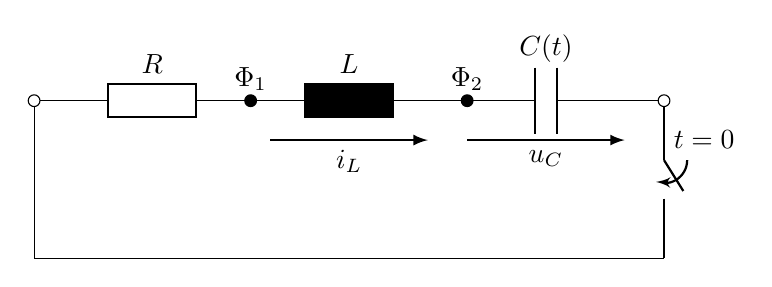
\begin{tikzpicture}[]

        % Vertical lines and empty circles
        \draw (0,2) -- (0,0);
        
        \draw (8,2) node[] {}
              to[closing switch, -] (8,0);
            \draw (8,1.5) node[right] {$t=0$};

        % Node in the middle of the line connecting R and L
        \draw (2.75,2) node[draw, circle, inner sep=1.5pt, fill=black] {};
        \draw (2.75,2) node[above] {$\Phi_1$};
        \draw (5.5,2) node[draw, circle, inner sep=1.5pt, fill=black] {};
        \draw (5.5,2) node[above] {$\Phi_2$};
        % Horizontal line and components
        \draw (0,2) node[draw, circle, inner sep=1.5pt, fill=white] {}
              to[R=$R$] (3,2)
              to[L=$L$] (5,2)
              to[C=$C(t)$] (8,2) node[draw, circle, inner sep=1.5pt, fill=white] {};

        % Bottom horizontal connection
        \draw (0,0) -- (8,0);

        % Voltage arrows
        \draw[->, thick, >=latex] (3,1.5) -- (5,1.5) node[midway, below] {$i_L$};
        \draw[->, thick, >=latex] (5.5,1.5) -- (7.5,1.5) node[midway, below] {$u_C$};

    \end{tikzpicture}
    \caption{RLC soros rezgőkör.}
    \label{fig:rlc}
\end{figure}

A szimulációmat egy soros RLC körre végeztem (\ref{fig:rlc}. ábra). Az áramkör forrást ugyan nem tartalmaz, de nem energiamentes: $u_C(0) \ne 0$. További kezdeti feltételként
megszabtam még továbbá, hogy a tekercs energiamentes állapotban van ($i_L(0) = 0$).

A kondenzátor kapacitását az alábbi (\ref{ct}) időfüggvény írja le:

\begin{equation}
    C(t) = C_0 \left[1 + c \cdot \sin(\omega_p t)\right]
    \label{ct}
\end{equation}
, melynek deriváltja
\begin{equation}
    \frac{dC(t)}{dt} = {C}' = C_0 \cdot c \cdot \omega_p \cdot \cos(\omega_p t)
    \label{dct}
\end{equation}
, ahol $C_0$ a kondenzátor alap kapacitása, $c$ a kapacitás "pumpálás" amplitúdója, $\omega_p$ pedig a körfrekvenciája.

Ennek megfelelően az időfüggő kapacitású kondenzátor karakterisztikája a következő módon kapható:

\begin{equation}
    \begin{split}
        i_C(t) & = \frac{d}{dt}(C(t) \cdot u_c(t)) \\
        i_C(t) & = C(t) \cdot \frac{du_c(t)}{dt} + \frac{dC(t)}{dt} \cdot u_c(t)
    \end{split}
\end{equation}

\begin{equation}
    \boxed{i_C = C(t) \cdot u'_C + C' \cdot u_c(t)}
\end{equation}

\pagebreak

Ezzel és a hagyományos (konstans induktivitású) tekercs karakterisztikával ($u_L = L \cdot i_L'$) már a $\Phi_1$-es és a $\Phi_2$-es potenciálú
csomópontra (\ref{fig:rlc}) felírjuk a csomóponti egyenleteket:

\begin{equation}
    \begin{split}
        \frac{u_C + Li_L'}{R} + i_L = 0 \\
        -i_L+Cu'_C + C'u_C = 0
    \end{split}
\end{equation}
, melyekből az Állapotváltozós Leírás Normálalakja (ÁVLNA) könnyedén előállítható:
\begin{equation}
    \boxed
    {
        \begin{split}
                u'_C = \frac{i_L}{C} - \frac{C'u_C}{C} \\
                i'_L = -\frac{u_C}{L} - \frac{Ri_L}{L}
        \end{split}
    }
    \label{avlna}
\end{equation}

Ezzel megkaptuk a parametrikus oszcillátorunk állapotváltozóit (jelen esetben a kondenzátor $u_C$ feszültségét és a tekercs $i_L$ áramát)
leíró differenciálegyenlet-rendszert.

\section{Numerikus megoldás és szimuláció}

Az előállított differenciálegyenlet rendszert MATLAB környezetben könnyedén meg lehet oldani.

Először a kódban definiálom az ellenállás $R$ [Ohm], a tekercs induktivitás $L$ [Henry], az alapkapacitás $C_0$ [Farad],
a kondenzátor kezdőfeszültség $U_0$ [Volt] és a kapacitás pumpálás amplitúdó $c$ (esetlegesen a körfrekvencia $\omega_p$ [rad/s]) értékeket.
Ezekből a kód kiszámítja az $\omega_0 = 1 / \sqrt{L \cdot C_0}$ képlet alapján a soros RLC kör sajátfrekvenciáját és alapesetben beállítja a kapacitáspumpálás körfrekvenciáját
ennek a kétszeresére $\omega_p = 2 \omega_0$:

\begin{lstlisting}
% Parameterek SI-ben
R = 5;                      % Ellenallas (ohm)
L = 10e-3;                  % Induktivitas (H)
C0 = 10e-6;                 % Alapkapacitas (F)

c = 0.4;                    % Kapacitas valtozas (pumpalas) amplitudoja
U0 = 5;                     % Kezdo feszultseg (V)

omega_0 = 1/sqrt(L*C0);     % Rezonancia korfrekvencia (rad/s)
omega_p = 2 * omega_0;      % Pumpalas korfrekvencia (rad/s)
\end{lstlisting}

Ezután a kapacitás időfüggvényét és az analitikus úton kapott deriváltját, illetve az ÁVLNA differenciálegyenleteit definiálom:

\begin{lstlisting}
% Differencialegyenlet megoldasa
% Allapotvaltozok: x(1) = U_C (kondenzator feszultsege), x(2) = I (aram)
C_t = @(t) C0 * (1 + c * sin(omega_p * t)); % Kapacitas idofuggvenye
dC_dt = @(t) c * omega_p * C0 * cos(omega_p * t); % Kapacitas idoderivaltja

dxdt = @(t, x) [
    1/C_t(t) * x(2) - dC_dt(t)/C_t(t) * x(1); % dU_C/dt = 1/C(t) * I - dC/dt/C(t) * U_C
    -x(1)/L - R/L * x(2)                      % dI/dt = -U_C/L - R/L * I
    ];
\end{lstlisting}

Végül a szimuláció időtartama, a kezdeti feltételek ($u_c(0)$ és $i_L(0)$) és az \texttt{ode45} solver opciói beállításra kerülnek és meghívom az \texttt{ode45} megoldó függvényt.

\begin{lstlisting}
% Idotartomany
tspan = [0, 30e-3]; % Szimulacio idotartama (s)

% Kezdeti feltetelek
x0 = [U0; 0]; % U_C(0) = U0, I(0) = 0

% ode45 opciok (RelTol, AbsTol, MaxStep)
options = odeset('RelTol',1e-8,'AbsTol',1e-10,'MaxStep',1e-6, 'Stats', 'on', 'OutputFcn', @odeplot);

% Megoldas ode45-tel
[t, x] = ode45(dxdt, tspan, x0, options);
\end{lstlisting}

A szimuláció időtartamát akár automatikusan is be lehetne állítani az rezgőkör időállandója alapján ($3\tau \dots 10 \tau$), de ennek megválasztását
a felhasználóra hagyom. Az \texttt{ode45} függvény alapesetben a Runge-Kutta-módszerrel oldja meg az átadott differenciálegyenlet-rendszert, ám tapasztalataim
alapján a beépített funkciója gyakran túl nagy lépésközt választ, ezért szükséges specifikálni a \texttt{MaxStep} maximum időlépési közt a szimuláció
hoszabb időtartamú stabilitása miatt (alapesetben ez 1 ns-ra van választva), illetve hasznos és érdekes látni, ahogy a solver folyamatában oldja az egyenleteket,
így a \texttt{'Stats', 'on', 'OutputFcn', @odeplot} opciók is alapesetben definiálva lettek (természetesen ezek nem feltétlenül szükségesek a szimuláció működéséhez).

A végső eredmény, amely a \texttt{[t, x]} vektor(ok)-ban vannak tárolva ki is lesznek plotolva.

\section{Elemzés a szimuláció segítségével: a körfrekvenciák és a működés viszonya}


\end{document}